\documentclass[../main.tex]{subfiles}

\begin{document}
\chapter{Real-Time Operating Systems}

\section{Scheduling}
The \define{scheduling problem} in a real-time operating system is finding a suitable order of task execution, more specifically one that satisfies the real-time constraints.
When dealing with \textit{hard real-time systems}, these constraints need to be satisfied, no matter what. The problem is twofold:

\begin{enumerate}
	\item \textbf{Are there schedules that satisfy the constraints?} \\
	Can deadlines be maintained? What's the worst case processing time? To answer these questions processing time must be bound, resources must be available and interaction between processes possible.
	\item \textbf{If such schedule(s) exist, find one!}
\end{enumerate}

\subsection{Classic Real-Time Scheduling}
\subsubsection{Static Scheduling}
With static scheduling all decision are made \textbf{before the system is started}. Schedulability analysis is performed statically without the system running. Usually the program will consist of a loop that performs all tasks in sequence. Sometimes tasks are only executed a limited amount of times each iteration. The loop runs either continuously or is started every clock tick. The last approached is used by most programmable logic controllers.
\\\\
Interrupts are often disabled, since they are not really necessary when we know on beforehand what's going to happen. If there are interrupt routines, they are taken into account as high priority periodical tasks which run at the highest possible repetition rate of the interrupt.
\\\\
Static scheduling is only suitable for simple and immutable systems. However, system that do not change do not exist, so when anything changes the scheduling analysis needs to be repeated. This can be a problem, for example when a component needs urgent replacement by a non-identical one.

\subsubsection{Dynamic Scheduling}
Dynamic scheduling is used when static scheduling is not appropriate.
\begin{enumerate}
	\item Perform a rough static scheduling analysis to evaluate the \textbf{worst-case processing time}. Also verify that, unless the scheduler makes a gross fault, the scheduler will be able to satisfy all timing constraints.
	\item Let a dynamic scheduler choose the order of execution of tasks.
	\item Unless it can be proven that the scheduler always makes the right choice, test should cover as many situations as possible in order to verify timing constraints are met.
\end{enumerate}

Every mutli-tasking operating system (real-time or not) includes a scheduler. The classical qualities expected from the scheduler in an ordinary operating system consist of :
\begin{itemize}
	\item \definebf{Fairness}: All tasks should receive a fair share of computing time.
	\item Optimization of the \textbf{mean response time}
	\item Optimization of \textbf{available processing time}
\end{itemize}
The real-time scheduler on the other hand has only one goal: guarantee that all real-time tasks will be finished before their deadline.
\\\\
Independent of whether the scheduler is real-time, they can be divided in two classes:
\begin{itemize}
	\item \textbf{Non preemptive}: when the a task is allowed to run, the scheduler waits for the task to finish before allowing another task to run.
	\item \textbf{Preemptive}: the scheduler may suspend the execution of a running task when it judges appropriate.
\end{itemize}

\begin{blockquote}
At first sight, a preemptive scheduler who can suspend tasks in favor of more urgent tasks will obtain better results. This is not always the case because resource conflicts can arise. If  the lower priority task has locked a resource which is needed by the more urgent task, this tasks may not be suspend before this resource is freed. If this is not the case, the higher priority task would simply block, waiting for the resource.
\end{blockquote}

There are 3 techniques available for selecting the next task to run on a non-periodic real-time system.
\begin{itemize}
	\item \index{Task Selection!Fixed Priorities} \textbf{Fixed Priorities} \\
	Each task is assigned a fixed priority which has to be chosen with care. The priority should incorporate the urgency as well as the criticality of the task. The scheduler always selects the task with all its resource available and the highest priority. This technique is easy to implement but if there's always a task with a high priority, the lower priority task might be overrun.

	\item \index{Task Selection!Closest Deadline First} \textbf{Closest Deadline First} \\
	The scheduler selects the task closest to its deadline. This implies the deadline of each task is known. This can only be known at run time.

	\item \index{Task Selection!Least Laxity First} \textbf{Least Laxity First} \\
	This scheduling technique selects the tasks with the lowest latency. If the task is started after that time, it cannot respect its deadline. The deadline and maximum execution times of tasks must be known.
	\begin{center}
		$	\textit{laxety} = t_{\textit{deadline}} - t_{\textit{now}} - \textit{task execution time}$
	\end{center}
	\end{itemize}

\subsubsection{Priority Inheritance}
A scheduler always selects one of the tasks that are ready to run, which means all its resources are available. This can be a problem when several tasks need the same resource and one tasks needs the resource without it being released between subsequent runs.

\begin{exmp}
A task could have to send a message over the network to another machine. As long as the message is not entirely transmitted, no other task may send over the network. If not, what would travel on the network would be the beginning of the first message, followed by the second message, followed by the end of the first message. The resulting traffic would not make any sense.
\end{exmp}

To avoid the problem mentioned, a task can use a \textbf{mutex} on the resource he needs. If the mutex is free, the task can reserve it for itself, otherwise it waits for it to be released. The task is then suspended and only restarted when the resource is free.
\\\\
Consider the following problem, called the \textbf{priority inversion} as illustrated below.
\begin{exmp}
There are 3 tasks $T_i$ close to their deadlines with priority $i$. If there were no resource problems the scheduler would select them in the following order: $T_1, T_2, T_3$. Task $T_1$ and $T_3$ need the same resource. Assume that $T_3$ is running and using the resource and the scheduler learns that $T_1$ and $T_2$ must be run urgently. This is what would happen:
\begin{enumerate}
	\item The scheduler suspends $T_3$ which is holding the resource.
	\item Since $T_1$ cannot run, $T_2$ is chosen.
	\item After $T_2$ only $T_3$ is available and the scheduler consequently activates it.
	\item Finally $T_1$ is run as soon as $T_3$ finishes.
\end{enumerate}
Because of the resource,$T_2$ has been executed before T1 instead of the opposite: This is called the priority inversion problem. What should have happened is that $T_3$ was allowed to finish so that the resource was released and $T_1$ could run before $T_2$.
\end{exmp}
To enforce correct behaviour, \definebf{priority inheritance} is used. The list of resources needed by each task is known by the scheduler. When a lower priority task is running and uses a necessary resource, that task temporarily inherits the more urgent task's priority untill the resource is freed.
\\\\
Notes:
\begin{itemize}
	\item The higher the number of tasks with different priorities who need the same resource, the more often this problem arises.
	\item The longer a task uses a resource, the more this task will slow down a higher priority task even with our solution.
	\item If several tasks need a same set of resources at the same time, they must lock all resources atomically. If not, a deadlock might occur.
\end{itemize}

\subsubsection{Effect of Interrupts}
An interrupt management system behaves like a preemptive scheduler with fixed priorities. It shares the responsibility of allocating the computer's processing time with the scheduler but is hierarchically of greater importance.
\\\\
The scheduler of the operating system can only allocate the processing time left by the interrupt routines. If we aim to have the system mainly managed by the scheduler, interrupt routines should be very short. The interrupt should inform the scheduler but the latter will have to decide for itself to activate it or not.
\\\\
For timing calculations, one can try to estimate the maximum amount of time lost by interrupt routines and add this value to the task's own processing time.

\subsubsection{Periodic Tasks}
An interesting special case is that of systems that only  have periodic tasks but with a different value of periodicity.
If all tasks are independent and if it is possible to satisfy all timing constraints then the scheduler that always activates the task with the highest repetition rate will meet all the deadlines.
This approach is called \definebf{rate monotonic scheduling}. Unfortunately, situations where all tasks are independent are rare.

\subsection{Reservation Scheduling}
Rather than executing the scheduling algorithm every time a new task must be selected, \textbf{Reservation Scheduling} will make this choice on beforehand, as soon as the necessary information is available.

If it is possible to schedule a task between the current time and the moment there will be no known tasks left to execute, a schedule is prepared. If the previous is not possible, the scheduler decides what tasks should be sacrificed, based on their importance (criticality) rather than their urgency. Sacrificed tasks may be replaced by shorter ones aimed at limiting the impact of sacrificing the task. Tasks that are urgent but not critical may simply be dropped.

\begin{exmp}
The considered system is an airplane. An example of a shorter task to replace the sacrificed task is the case where, if the plane cannot be saved, he is ejected. An example of a dropped task is fuel optimization when it must be leveled urgently.
\end{exmp}

This scheduling approach is implemented in two parts:
\begin{enumerate}
	\item \textbf{Pre-Scheduler} prepares a scenario.
	\item \textbf{Dispatcher} activates tasks according to the scenario. It resembles the static scheduler, it has nothing to decide.
\end{enumerate}

\subsubsection{Reservation Scheduling Types}

There are two types of reservation schedulers for both the scheduler and the dispatcher. We're considering the scheduler first.\\\\
The first variant has the pre-scheduler simply check that the timing constraints can be satisficed and accepts or rejects tasks. The dispatcher works like a classical dynamic scheduler. This introduces the risk that the fact that there is one schedule that meets all timing requirements does not mean that all possible schedule do. The dispatcher could still make the wrong choice.
\\\\
The second variant has the pre-scheduler build itself a schedule that it has proved to meet the requirements. The dispatcher then executes it without changing anything. This variant is considered to be the best.
\\\\
The dispatcher can be preemptive or non preemptive. In the first case the pre-scheduler must decide when the dispatcher will suspend each running task. The problem here is that there must be a way to make sure a long task is not cut at the wrong moment. The solution is making use of \textbf{critical sections}. The scheduler then knows not to cut the task at that time.
\\\\
When non preemptive scheduling is used no task can have a shorter guaranteed response time than the duration of the longest task.
\\\\
In conclusion there are 3 acceptable solutions:
\begin{itemize}
	\item \textbf{Non preemptive with short tasks}. It's up to the programmer to decide where to cut.
	\item \textbf{Preemptive with a scheduler that knows were not to cut}. The programmer must indicate these sections.
	\item \textbf{Preemptive with short critical sections}. Sections are so short that the chance of them being cut is negligible.
\end{itemize}

\subsubsection{Assessment of Reservation Schedulers}
Reservation schedulers take into account both urgency and criticality of a task. A classic dynamic scheduler will always select the most urgent task, but this is not always the best choice. Reservation schedulers make their decision earlier so they can balance their decision based on all known factors. They can decide to sacrifice a an urgent task for a more important one.
\\\\
Why don't all real-time systems use reservation schedulers? This is because if the system has the necessary resources to never miss a deadline, a classic scheduler is able to do the job. However, since more and more real-time systems are computer controlled, overdimensioning the controlling computers is not always a good idea, especially not when they are battery operated. Reservation schedulers may in that case be the better choice.

\section{Example: MicroC/OS-II}
\textit{Information presented in this section is based on the book of Jean Labrosse, MicroC/OS-II, The Real-Time Kernel, Second Edition, ISBN-13:978-1-57820-103-7. The presentation is different.}
\\\\
MicroC/OS-II is a commercial product of Micrium. However, higher education institutions may use, without charge for teaching purposes, as well the sources of this software as the executable programs themselves.
\\\\
In MicroC/OS-II, each task has a different priority (a value between 4 and 60, 4 being the highest and 60 the lowest) and the scheduler is a simple dispatcher that will always launch the highest priority task. This may look rather primitive, but it is actually rather versatile because the priority of tasks may be changed dynamically. MicroC/OS-II uses that feature internally to avoid priority inversion, but it could also be used to give a task the role of pre-scheduler. However, using the same value to identify a task and his priority can be a nuisance to handle if the priority changes relatively often.
\\\\
The operating system is simply linked with the application: the main() function of the program is the OS; the code of application tasks is implemented as C functions called by this main().

\includelisting{microcosii.c}{style=cstyle, label=l:microc}

The private memory areas of each task must be declared as a global static variable, arrays are used to store the stack of tasks.
Variables shared by several tasks (there is none in this example) must also be declared as global static variables.
The EVENT structures associated with events that tasks can be waiting for must be declared as global static variables too:
\begin{itemize}
	\item Interrupts
	\item Mutex and semaphores,
	\item Task synchronization
\end{itemize}
The \texttt{main()} function initializes the operating system and the data structures used and one or several tasks. Each task can launch other tasks. The last operation of \texttt{main()} is to start the scheduler. Initializing a task means associate with that task:
\begin{itemize}
	\item The function can execute the tasks.
	\item A pointer to the data structure of the task (where static variables are stored)
	\item A pointer to the top of the task's stack
	\item The initial priority of the task
\end{itemize}
All this is performed by the function \texttt{OSTaskCreate()}. The rest of the program consists of the functions corresponding to the tasks and of other functions.

\subsection{Tasks in MicroC/OS-II}
The code of the functions inside the body of a task in MicroC/OS-II must respect two constraints:
\begin{enumerate}
	\item \textbf{It may never reach the final bracket of the function nor call \lstinline{return()}.} Indeed, each tasks has its own stack, and the function that is the body of a task is at the absolute top of this stack: there is nothing above, so, it is impossible to return to a calling program. A way to satisfy this requirement is to include in this function, possibly after an initialization phase an infinite loop. Another option is calling a self destruction function when the task has finished its job \texttt{OSTaskDel(OS\_PRIO\_SELF);}.
	\item \textbf{It may not run continuously.} Since  MicroC/OS-II is preemptive, if a task could run continuously, no task of lower priority would ever be allowed to run.
\end{enumerate}
If you want a task to be allowed to run as often as possible you could give it the lowest priority.
If the application must include several such tasks, a function should be written for each one and the lowest priority task might be an infinite loop calling all these functions.
However, it should be noted that it is rarely useful to let a task run continuously.
Running the function more frequently than needed therefore is wasted activity.
It is often sufficient to wake the task up a certain amount of times per second and let it go back to sleep afterwards.

\subsubsection{Task States in MicroC/OS-II}
\begin{figure}[H]
    \centering
    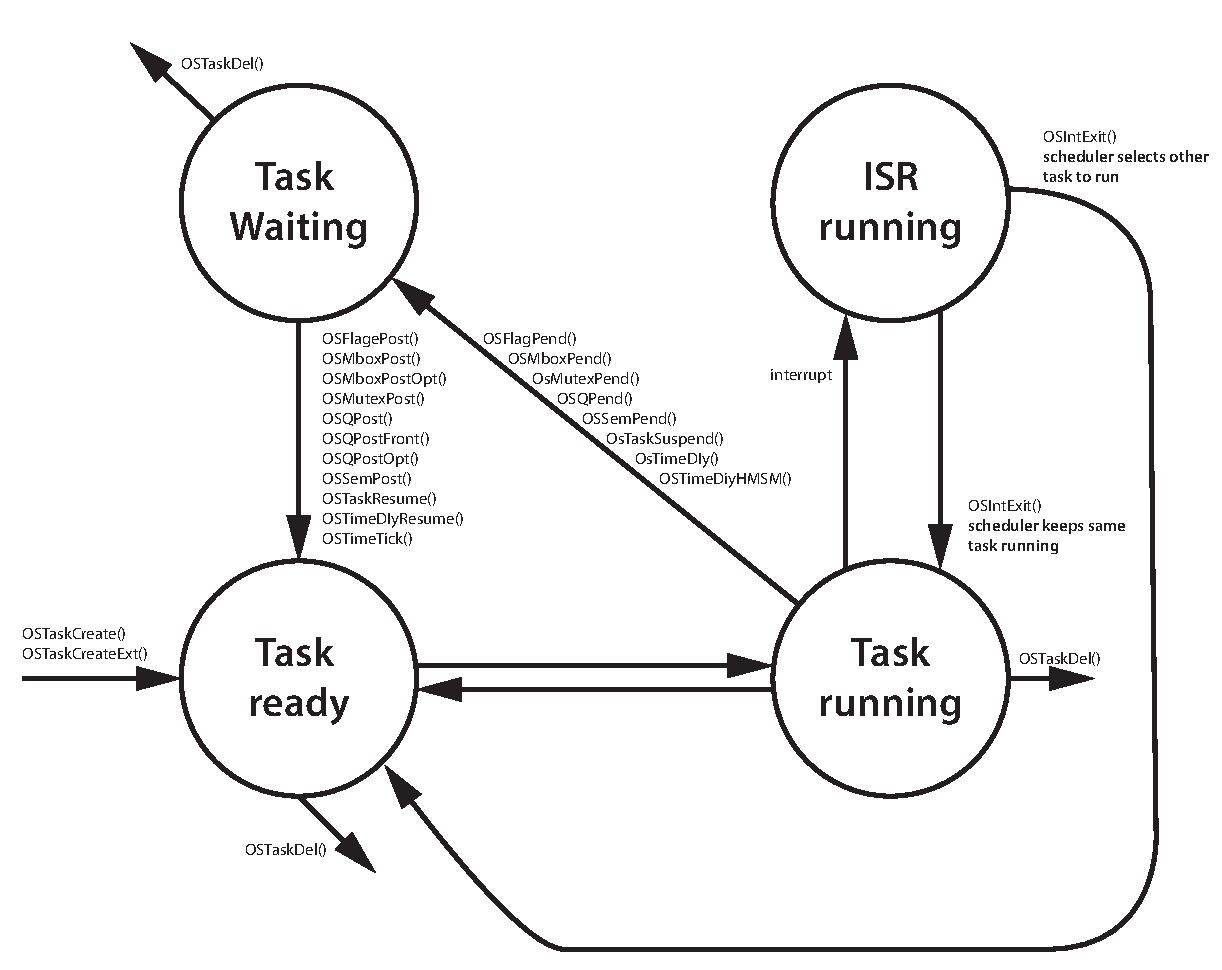
\includegraphics[width=\textwidth]{microCOS_states.pdf}
    \caption{MicroC/OS-II States}
    \label{mcosii}
\end{figure}

A task is in either of the \define{task states} shown in figure \ref{mcosii}.
\begin{itemize}
	\item When the task is created, the task is \textbf{ready} to run.
	\item When the task is selected by the scheduler it's in the \textbf{running} state.
	\begin{itemize}
		\item The task can be suspended by an interrupt.
		\item The task can switch to the \textbf{waiting} state because it's waiting or suspended by another task.
	\end{itemize}
	\item When the task is suspended due to an interrupt, the task switches to the \textbf{ISR} state. An \textit{Interrupt Service Routine} is a sequence of assembly language instructions that saves the processors registers on the stack and calls a C function or runs assembly code that:
	\begin{itemize}
	\item Warns the OS that an ISR starts by calling \texttt{OSIntEnter();}.
	\item Acknowledges the interrupt request on the interface to the interrupting device in order to clear the request.
	\item May reset the interrupt mechanism, that was temporarily deactivated by the hardware at the start of the ISR.
	\item Performs the appropriate processing according to the event announced by the interrupt.
	\item Warns the OS when it has finished by calling \texttt{OSIntExit();}. This function verifies whether there was a  higher priority task waiting. If this is the case the processor proceeds with this new task and puts the current one in the \textbf{ready} state.
	\end{itemize}
\end{itemize}

\subsubsection{The Main Task Management Functions}
The tasks of a real-time application generally require to cooperate with each other.
In order to do this in an organized manner, we need two techniques: \index{Mutual Exclusion!in MicroC/OS-II} \textbf{mutual exclusion} to gain exclusive access to a shared resource and a \index{Rendez-vous!in MicroC/OS-II| see {Barrier}}\textbf{rendez-vous} or \definebf{barrier} to meet each other after each task has completed.

\paragraph{Mutual Exclusion} The most useful service offered by MicroC/OS-II is the mutual exclusion \textbf{mutex} which is associated with each shared resource. When a task wants to obtain a mutex that is not free, it waits. It's also possible to check the availability of the mutex without moving to the waiting state. Priority inheritance is supported.

\paragraph{Barrier} Event Flags organize the \textit{rendez-vous} between tasks. They are sets of bits (8/16/32) that may be set to 0 or 1 by tasks or ISRs. Tasks wait for a given pattern of bits to appear. Because this mechanism is so general it allows for complex conditions.

\section{Peripherals and IO}
System services will be as simple as possible.
The more complex the system is, the harder it is to guarantee its constraints.
This approach is called the \defineabrv{Reduced Instruction Set Computing}{RISC} Philosophy.
\\\\
From a technical point of view interrupts routines are short to avoid interference with scheduling. Disk management, if any, tries to avoid disk access in actions that must be performed before a hard deadline. Contiguous files have sometimes been recommended for real-time systems. Their inconvenience however, exceed their advantages: each one must be created with the maximum size (which is a waste of space) and there is no advantage if blocks are read one by one.

\subsection{I/O with MicroC/OS-II}
MicroC/OS-II is a portable operating system. It consists of architecture independent and architecture dependent functions. Porting MicroC/OS-II means rewriting the latters; these are generally not visible by the application programs: they are underneath the architecture independent functions.
\\\\
I/O functions are the exception: they are architecture dependent but visible by application programs. They are not part of the MicroC/OS-II distribution because they can differ as well by their interface as by their implementation in each application. They must thus be written by the application developper.



\section{Communication}
There are 3 ways to organize inter-process communications:
\begin{itemize}
	\item \textbf{Shared Data}: requires a mutex to guarantee data integrity.
	\item \textbf{Messages}: require a lot of overhead.
	\item \textbf{Unstructured Flows}: requires correct interpretation.
\end{itemize}
The communication model should not be mistaken for its implementation. The message system can be implemented for example using shared memory.
\\\\
The message model is easy to implement and has the advantage that it is asynchronous: the logistics are handled by the system, thus no need of mutex like for shared data.

\subsection{Communication with MicroC/OS-II}
MicroC/OS-II functions allow 3 types of \index{Task Communication! in MicroC/OS-II} task communications, all based on shared data structures but corresponding either to a shared data model or a message model.

\subsubsection{Communication by Shared Data}
Shared data structures are declared, for instance, as static global variables. To avoid interference between tasks, mutexes can be used to reserve exclusive access when needed.

\subsubsection{CMailbox Communication}
MicroC/OS-II provides a service called \textbf{mbox}, allowing to transfer a pointer to a data structure from one task to another. They allow transferring the permission to access  the pointed data structure from one task to another.


\subsubsection{Communication by messages queue}
The mboxes allow synchronizing a task on arrival of data produced by another task. However, because only 1 message at a time can be in a mbox, the sender (producer) can run ahead of the receiver (consumer). This is a common problem in a data processing system.
Message queues are a solution to this problem. Instead of a pointer to a message, they include a pointer to an array of pointers to messages. Like in any queue, the first message in the queue is the first message received.

\section{Time Management and Synchronization}
We expect a good clock to be \textbf{measurable}, \definebf{chronoscopic} (increasing monotonously and without discontinuities), to have a known precision and to be fault tolerant. In a centralised system, there is no real problem if the quartz is sufficiently precise and stable. A clock can be derived from this and all times can be measured with this clock.

\subsection{\index{Time Management!with MicroC/OS-II} Time Management with MicroC/OS-II}
MicroC/OS-II includes a few time related functions based on regular interrupts of a timer. These interrupts are called \textbf{ticks}. At each tick, a 32 bit counter is incremented. If ticks happen every millisecond, there will be $85.4 10^6$ a day. This counter will reset to 0 after a little less than 50 days.

\subsection{Clocks in Distributed Systems}
Computer clocks are based on quartz oscillators that provide a stable frequency.
However, although stable, the frequencies of different quartz oscillators are never identical.
In order to \index{Time Synchronization} synchronize clocks, a mean time must be defined.
\\\\
Clock adjustments must be progressive: increase the rate of slow clocks and decrease that of fast clock. Setting the time is no option since that would invalidate the chronoscopic property. Doing this might require a special electrical circuit.
\\\\
\subsubsection{Fault Tolerant Average}
The \defineabrv{Fault Tolerant Average}{FTA} Algorithm is designed to synchronize clocks in a distributed system. There are two variants. The first ignores communication delays between systems, the second doesn't.
\\\\
When communication delays are ignored, each system broadcasts a message announcing its local time. Each system deduces the time-lag between its own clock and the others. The $k$ most different values from the mean are ignored. The correction to apply is the mean value of the time lags that have not been rejected.The correction is applied progressively, by slightly modifying the clock rate for a limited amount of time.
\[
C_i = \frac{1}{N-k}\sum^{N-k}_{j=1}D_ji
\]
\begin{exmp}
If $N = 2$ and $k=0$ then
\[
C_1 = \frac{D}{2} \;\;\; C_2 = -\frac{D}{2}
\]
\end{exmp}

The second variant does take communication delays into account. These delays trouble the correct measurement between the clocks: the time lag needs to be eliminated before calculating the mean time. We consider two cases: in the first one the delay is \textbf{symmetrical} and \textbf{predictable}. The second assumes the delay is predictable but \textbf{not symmetric}.

\paragraph{Symmetrical and Predictable Delay} We consider two systems: $A$ and $B$. System $A$ sends a message to $B$ including the time, measured in $A$, when the message was sent: $t_{a,0}$. Now $B$ receives the message at time $t_{b,1}$. With $D_{b,a}$ the time lag and $d_t$ the communication delay:
\[
t_{b,1} - t{a,0} = D_{b,a} + d_t = \Delta_l
\]
In the same way, $B$ sends a message including its transmission time $T_{b,0}$.
\[
t_{a,1'} - t_{b,1'} = D_{a,b} + d_t = \Delta_2
\]
No $A$ can compute
\[
\Delta_l + \Delta_2 = (D_{b,a} + d_t) + (D_{a,b} + d_t)
\]
Because $D_{b,a} = -D_{a,b}$ we know
\[
d_1 = \frac{\Delta_l + \Delta_2}{2}
\]
Ethernet is symmetrical but unpredictable because of collisions. So, the previous method could be applied if there were no collisions. Fortunately collision effects can easily be eliminated. The systems have to perform a few successive measurements of the time-lag instead of a single one. If the network is not overloaded, several results will be identical to the minimal value, which is the correct value.

\paragraph{Non Symmetrical Predictable Delay} Now we have to find the relation between the two communication delays.
\[
d_1( a \rightarrow b) = d_E + d_{t,ab} + d_R
\]
Here is
\begin{itemize}
	\item $d_E$ the processing delay at the sender
	\item $d_{rab}$ the network transmission delay
	\item $d_R$ the processing delay at the receiver
\end{itemize}
Using a second measurement from $A$ to $A$ yields
\[
d_p( a \rightarrow a) = d_E + d_{t,ab} + d_{t,ba} + d_R
\]
\[
\Delta_l + \Delta_2 = 2d_E + 2d_R + d_{t,ab} + d_{t,ba}
\]
\[
\Delta_{A \rightarrow A} = d_E + d_R + d_{t,ab} + d_{t,ba}
\]
According to the relative positions of the stations, one knows the relation between $d_{r,ab}$ and $d_{r,ba}$.

\subsubsection{Clock Resolution}
\index{Clock Resolution}
The following symbols are used:
\begin{itemize}
	\item $\Delta$: accuracy of the synchronization
	\item $g$: clock resolution
\end{itemize}
It's necessary that $| \Delta | \leq g \leq | 2 \Delta |$:
\begin{itemize}
	\item A higher resolution is not significant: it amounts only to adding insignificant decimals.
	\item A coarser resolution does not make fully use of the synchronization of the clocks.
\end{itemize}
In these conditions, one can identify the order of two events occurring on different sites, provided that they are at least two clock ticks apart.

\begin{figure}[H]
    \centering
    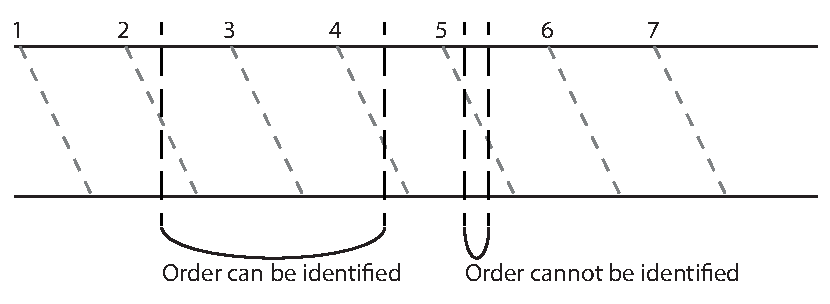
\includegraphics[width=0.8\textwidth]{timings.pdf}
    \caption{Clock Resolution}
    \label{clockres}
\end{figure}

\end{document}
